% exercise sheet with header on every page for math or close subjects
\documentclass[12pt]{article}
\usepackage[utf8]{inputenc} 
\usepackage{latexsym} 
\usepackage{multicol}
\usepackage{fancyhdr}
\usepackage{amsfonts} 
\usepackage{amsmath}
\usepackage{amssymb}
\usepackage{enumerate}
\usepackage{listings}
\usepackage{graphicx}
\usepackage{pdfpages}

% Shortcuts for bb, frak and cal letters
\newcommand{\E}{\mathbb{E}}
\newcommand{\V}{\mathbb{V}}
\renewcommand{\P}{\mathbb{P}}
\newcommand{\N}{\mathbb{N}}
\newcommand{\R}{\mathbb{R}}
\newcommand{\C}{\mathbb{C}}
\newcommand{\Z}{\mathbb{Z}}
\newcommand{\Pfrak}{\mathfrak{P}}
\newcommand{\Pfrac}{\mathfrak{P}}
\newcommand{\Bfrac}{\mathfrak{P}}
\newcommand{\Bfrak}{\mathfrak{B}}
\newcommand{\Fcal}{\mathcal{F}}
\newcommand{\Ycal}{\mathcal{Y}}
\newcommand{\Bcal}{\mathcal{B}}
\newcommand{\Acal}{\mathcal{A}}

% formating
\topmargin -1.5cm 
\textheight 24cm
\textwidth 16.0 cm 
\oddsidemargin -0.1cm

% Fancy Header on every Page
\pagestyle{fancy}
\lhead{\textbf{Programmierung for Engineers - Exercise 6}}
\rhead{Daniel Schäfer (2549458)\\ Dominik Weber (2548553)\\ Sina Vaghiri (2533563)}
\renewcommand{\headrulewidth}{1.2pt}
\setlength{\headheight}{60pt} 

\begin{document}
\pagenumbering{gobble}
\lstset{language=C}

\section*{Aufgabe 1.2}
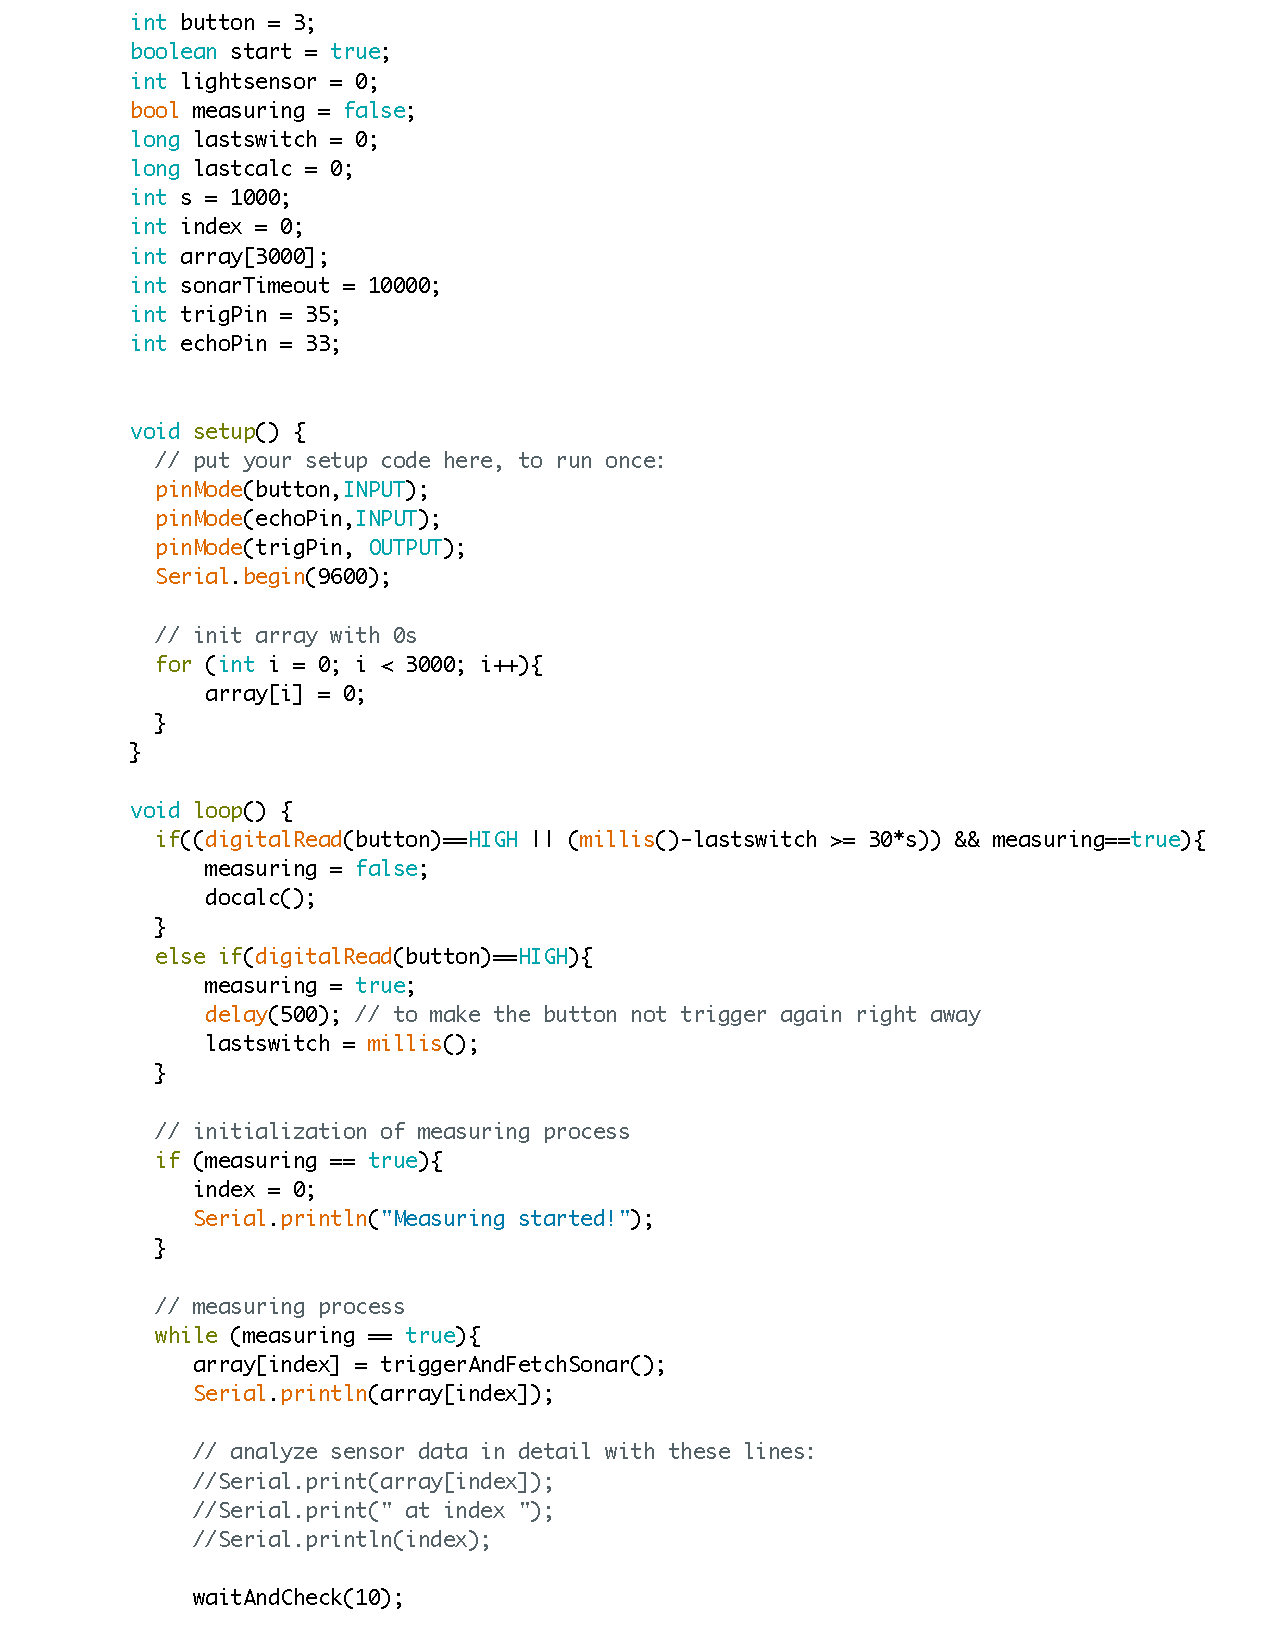
\includepdf[pages=-]{../Aufgabe12/Aufgabe12.pdf}


\section*{Aufgabe 1.3 - Bonus}
Die Werte sind unterschiedlich. Der Median besagt lediglich dass mindestens die Haelfte der Daten kleiner oder gleich sind als der Median und die haelfte der Daten groesser oder gleich dem Median sind. Der Median ist unempfindlich gegenuber Extremwerten. Der Durchschnitt dagegen ist empfindlich gegenueber Extremwerten (besonders bei sehr starken Ausreissern).
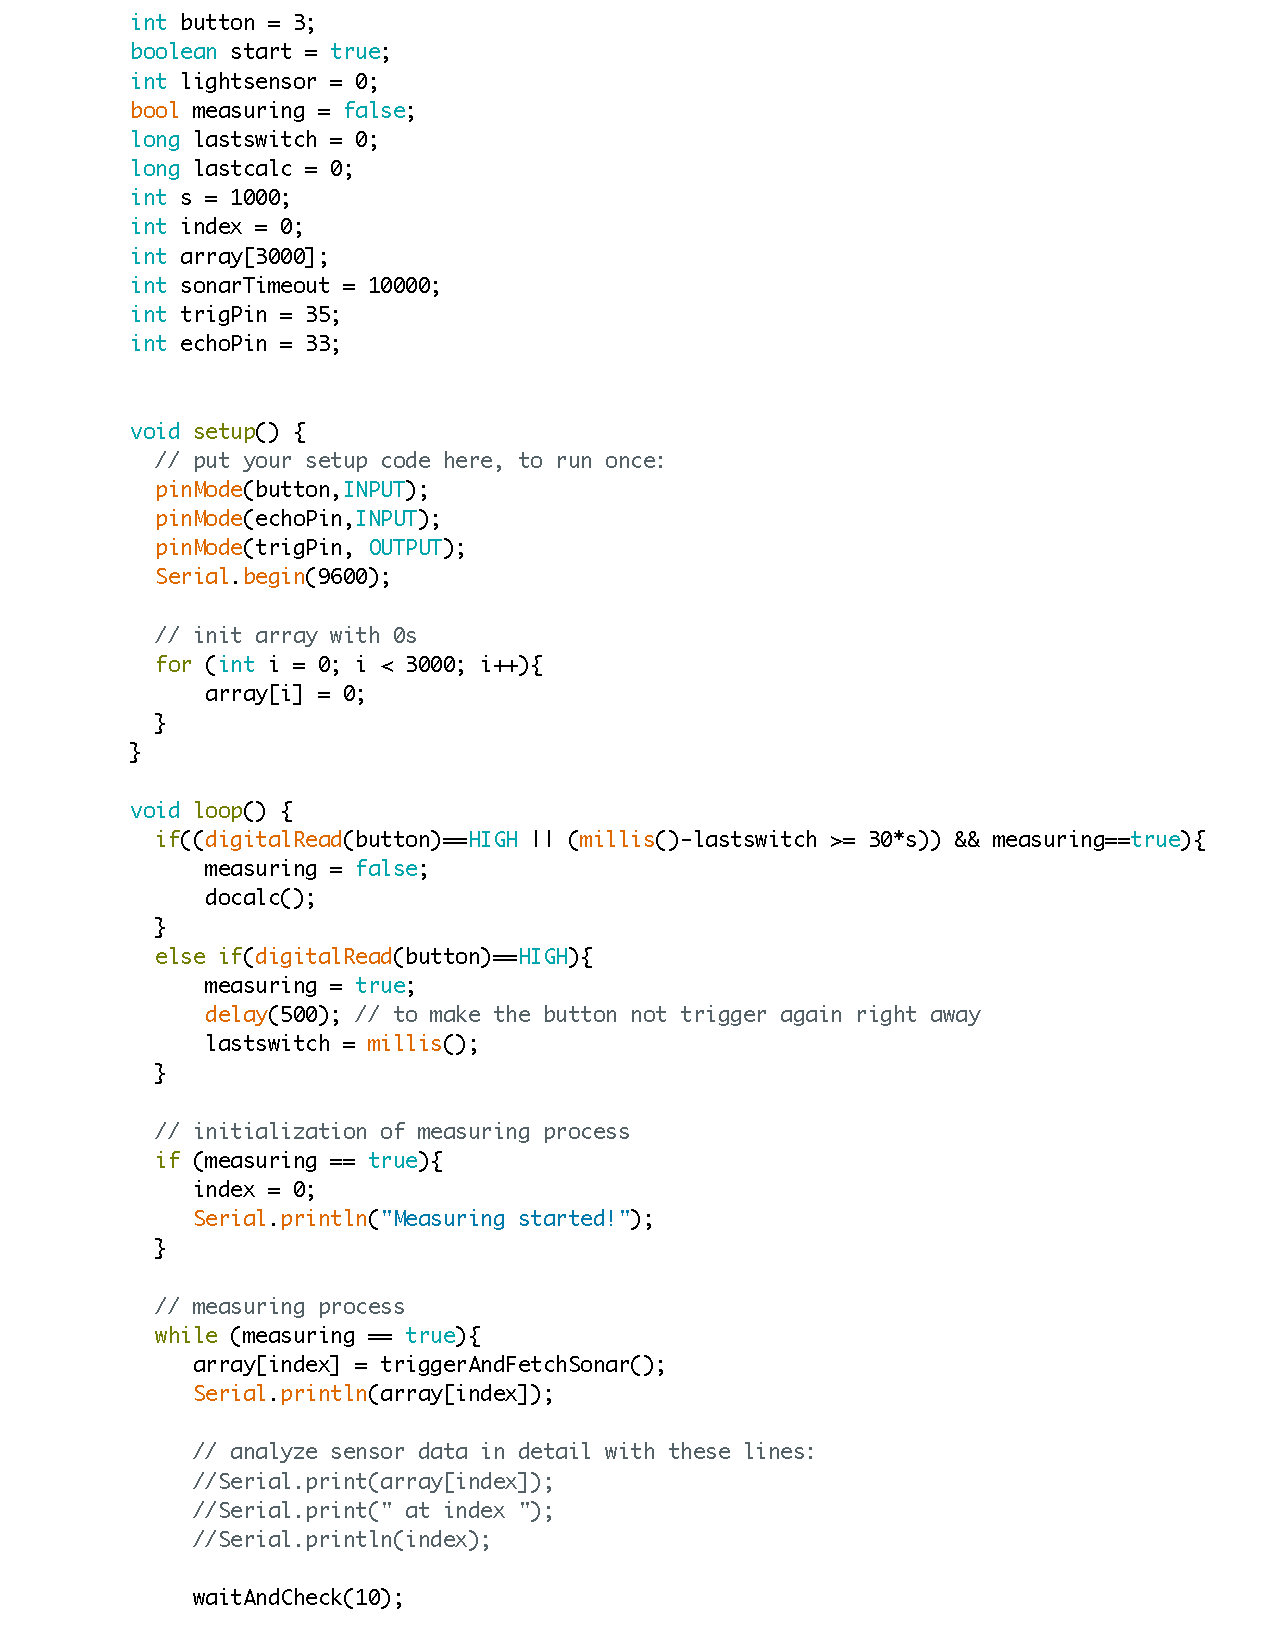
\includepdf[pages=-]{../Aufgabe13/Aufgabe13.pdf}


\section*{Aufgabe 1.4}
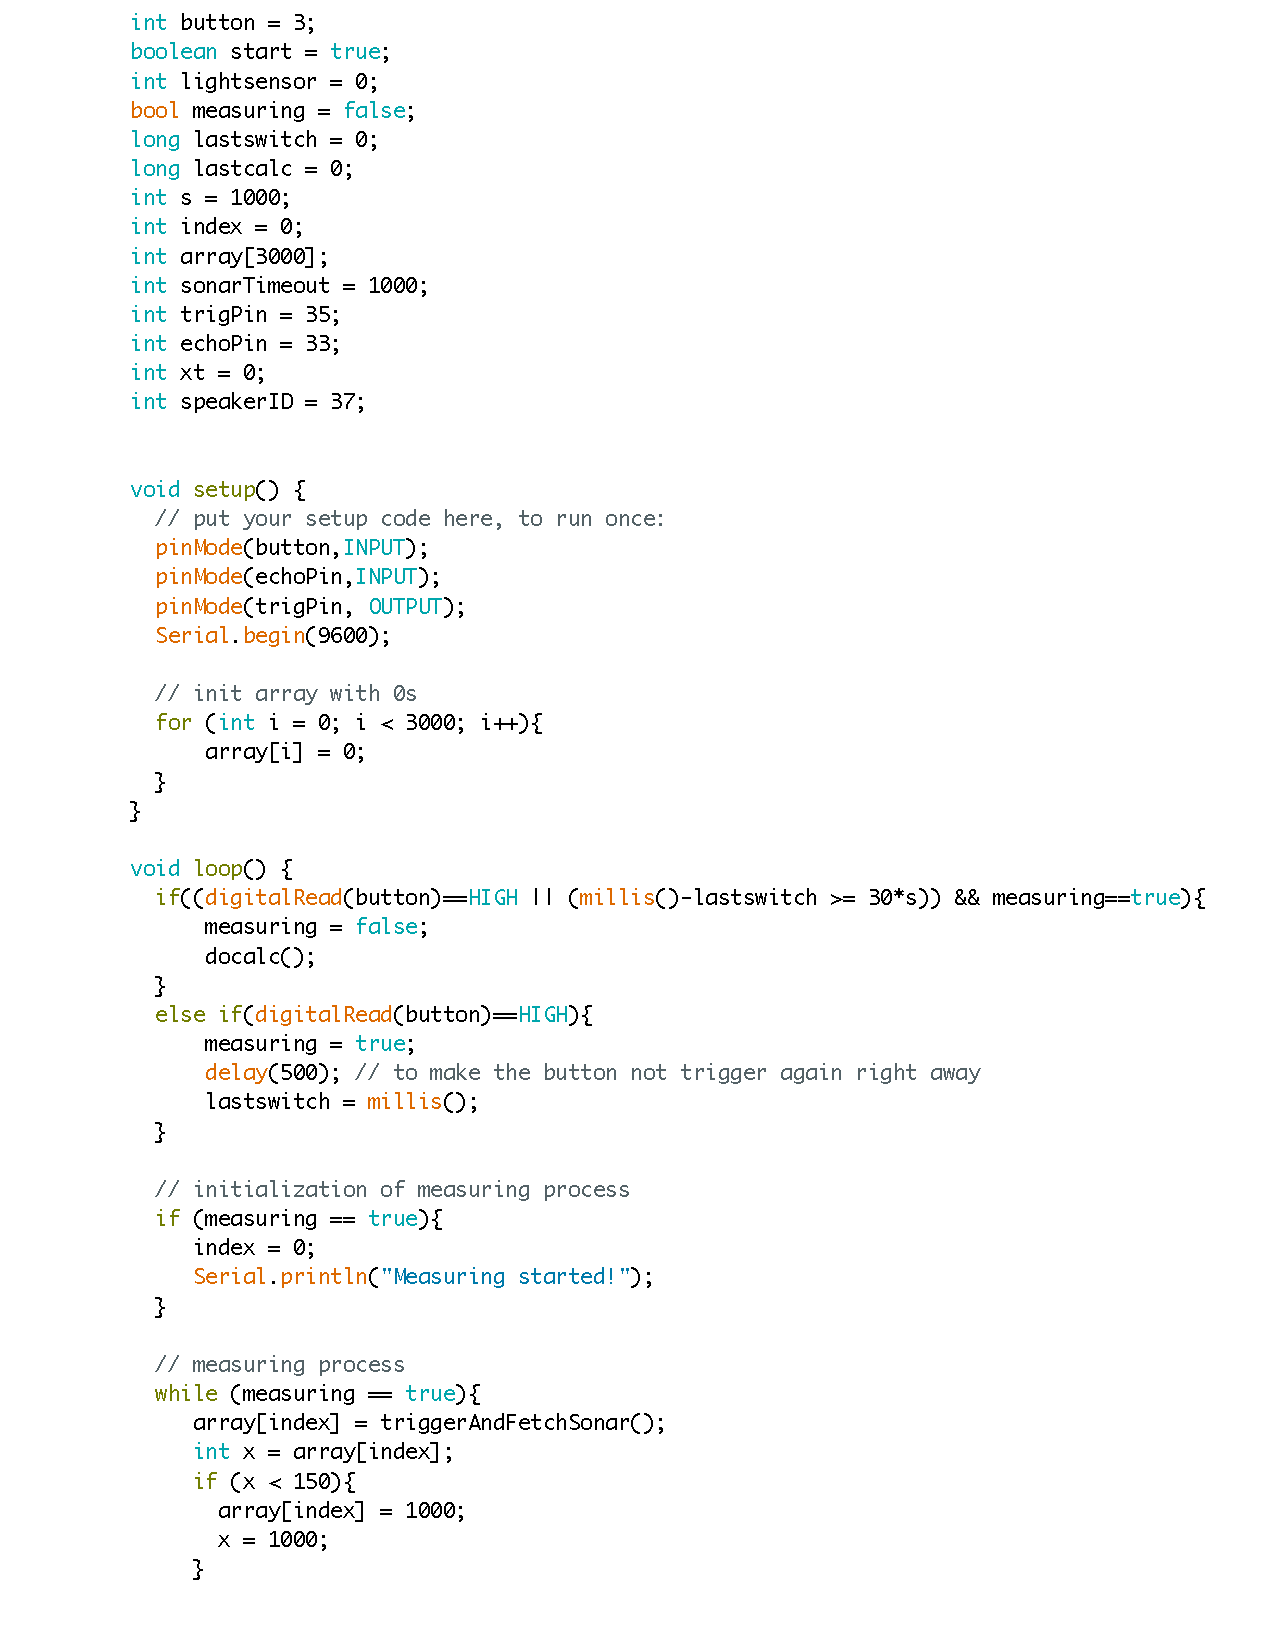
\includepdf[pages=-]{../Aufgabe14/Aufgabe14.pdf}

\section*{Aufgabe 2}

\textbf{Output unseres code:}\\
\begin{verbatim}
Laufzeitanalyse Unsorted
===============
 
Anzahl Elemente: 100
  Geschwindigkeit:
    InsertionSort : 5 ms
    MergeSort : 5 ms
Anzahl Elemente: 200
  Geschwindigkeit:
    InsertionSort : 17 ms
    MergeSort : 10 ms
Anzahl Elemente: 300
  Geschwindigkeit:
    InsertionSort : 37 ms
    MergeSort : 17 ms
Anzahl Elemente: 400
  Geschwindigkeit:
    InsertionSort : 65 ms
    MergeSort : 25 ms
Anzahl Elemente: 500
  Geschwindigkeit:
    InsertionSort : 98 ms
    MergeSort : 30 ms
Anzahl Elemente: 600
  Geschwindigkeit:
    InsertionSort : 143 ms
    MergeSort : 38 ms
Anzahl Elemente: 700
  Geschwindigkeit:
    InsertionSort : 200 ms
    MergeSort : 45 ms
Anzahl Elemente: 800
  Geschwindigkeit:
    InsertionSort : 267 ms
    MergeSort : 51 ms
Anzahl Elemente: 900
  Geschwindigkeit:
    InsertionSort : 327 ms
    MergeSort : 59 ms
\end{verbatim}

\newpage
\begin{verbatim}
Laufzeitanalyse Sorted
===============
 
Anzahl Elemente: 100
  Geschwindigkeit:
    InsertionSort : 1 ms
    MergeSort : 4 ms
Anzahl Elemente: 200
  Geschwindigkeit:
    InsertionSort : 1 ms
    MergeSort : 9 ms
Anzahl Elemente: 300
  Geschwindigkeit:
    InsertionSort : 0 ms
    MergeSort : 15 ms
Anzahl Elemente: 400
  Geschwindigkeit:
    InsertionSort : 1 ms
    MergeSort : 21 ms
Anzahl Elemente: 500
  Geschwindigkeit:
    InsertionSort : 1 ms
    MergeSort : 28 ms
Anzahl Elemente: 600
  Geschwindigkeit:
    InsertionSort : 1 ms
    MergeSort : 34 ms
Anzahl Elemente: 700
  Geschwindigkeit:
    InsertionSort : 1 ms
    MergeSort : 40 ms
Anzahl Elemente: 800
  Geschwindigkeit:
    InsertionSort : 1 ms
    MergeSort : 46 ms
Anzahl Elemente: 900
  Geschwindigkeit:
    InsertionSort : 2 ms
    MergeSort : 53 ms
\end{verbatim}

\newpage
\begin{verbatim}
Laufzeitanalyse Sorted but one
===============
 
Anzahl Elemente: 100
  Geschwindigkeit:
    InsertionSort : 0 ms
    MergeSort : 4 ms
Anzahl Elemente: 200
  Geschwindigkeit:
    InsertionSort : 0 ms
    MergeSort : 11 ms
Anzahl Elemente: 300
  Geschwindigkeit:
    InsertionSort : 0 ms
    MergeSort : 15 ms
Anzahl Elemente: 400
  Geschwindigkeit:
    InsertionSort : 1 ms
    MergeSort : 21 ms
Anzahl Elemente: 500
  Geschwindigkeit:
    InsertionSort : 2 ms
    MergeSort : 27 ms
Anzahl Elemente: 600
  Geschwindigkeit:
    InsertionSort : 1 ms
    MergeSort : 34 ms
Anzahl Elemente: 700
  Geschwindigkeit:
    InsertionSort : 2 ms
    MergeSort : 40 ms
Anzahl Elemente: 800
  Geschwindigkeit:
    InsertionSort : 2 ms
    MergeSort : 48 ms
Anzahl Elemente: 900
  Geschwindigkeit:
    InsertionSort : 2 ms
    MergeSort : 54 ms
\end{verbatim}

\newpage
\begin{itemize}
    \item 
        Auf einem unsortierten Feld ist mergeSort immer schneller (oder gleich schnell) als Insertion Sort. Wahrend der Unterschied bei kleinen Feldern noch relativ gering ist, steigt der Unterschied extrem stark an mit wachsender Feldgroesse.
    \item
        Ist das Feld jedoch entweder komplett oder fast komplett sortiert arbeitet InsertionSort extrem schnell. MergeSort dagegen ist kaum schneller als auf einem komplett unsortierten Feld.
    \item
        Dies war zu erwarten, da das splitten und mergen von Mergesort immer durchgefuehrt wird egal ob elemente schon sortiert sind oder nicht.
    \item
        Insertionsort dagegen muss im Fall sortiert ueberhaupt nichts tuen, es iteriert lediglich einmal ueber die Liste
    \item
        Im Fall alles sortiert ausser ein Element muss Insertionsort nur ein einziges Element der Liste bewegen, auch das ist extrem ``billig''.
    \item
        Besagte Sonderfaelle koennten in der Praxis natuerlich auftreten, jedoch wuerde ich behaupten, dass es unwahrscheinlich ist ein solches Szenario nicht im vorhinein zu verhindern. Also immer zu wissen ob ein Array bereits sortiert ist und bei dem hinzufuegen von Daten in ein sortiertes Array immer an die korrekte stelle einzufuegen, so dass die sortiert Eigenschaft erhalten wird.
\end{itemize}


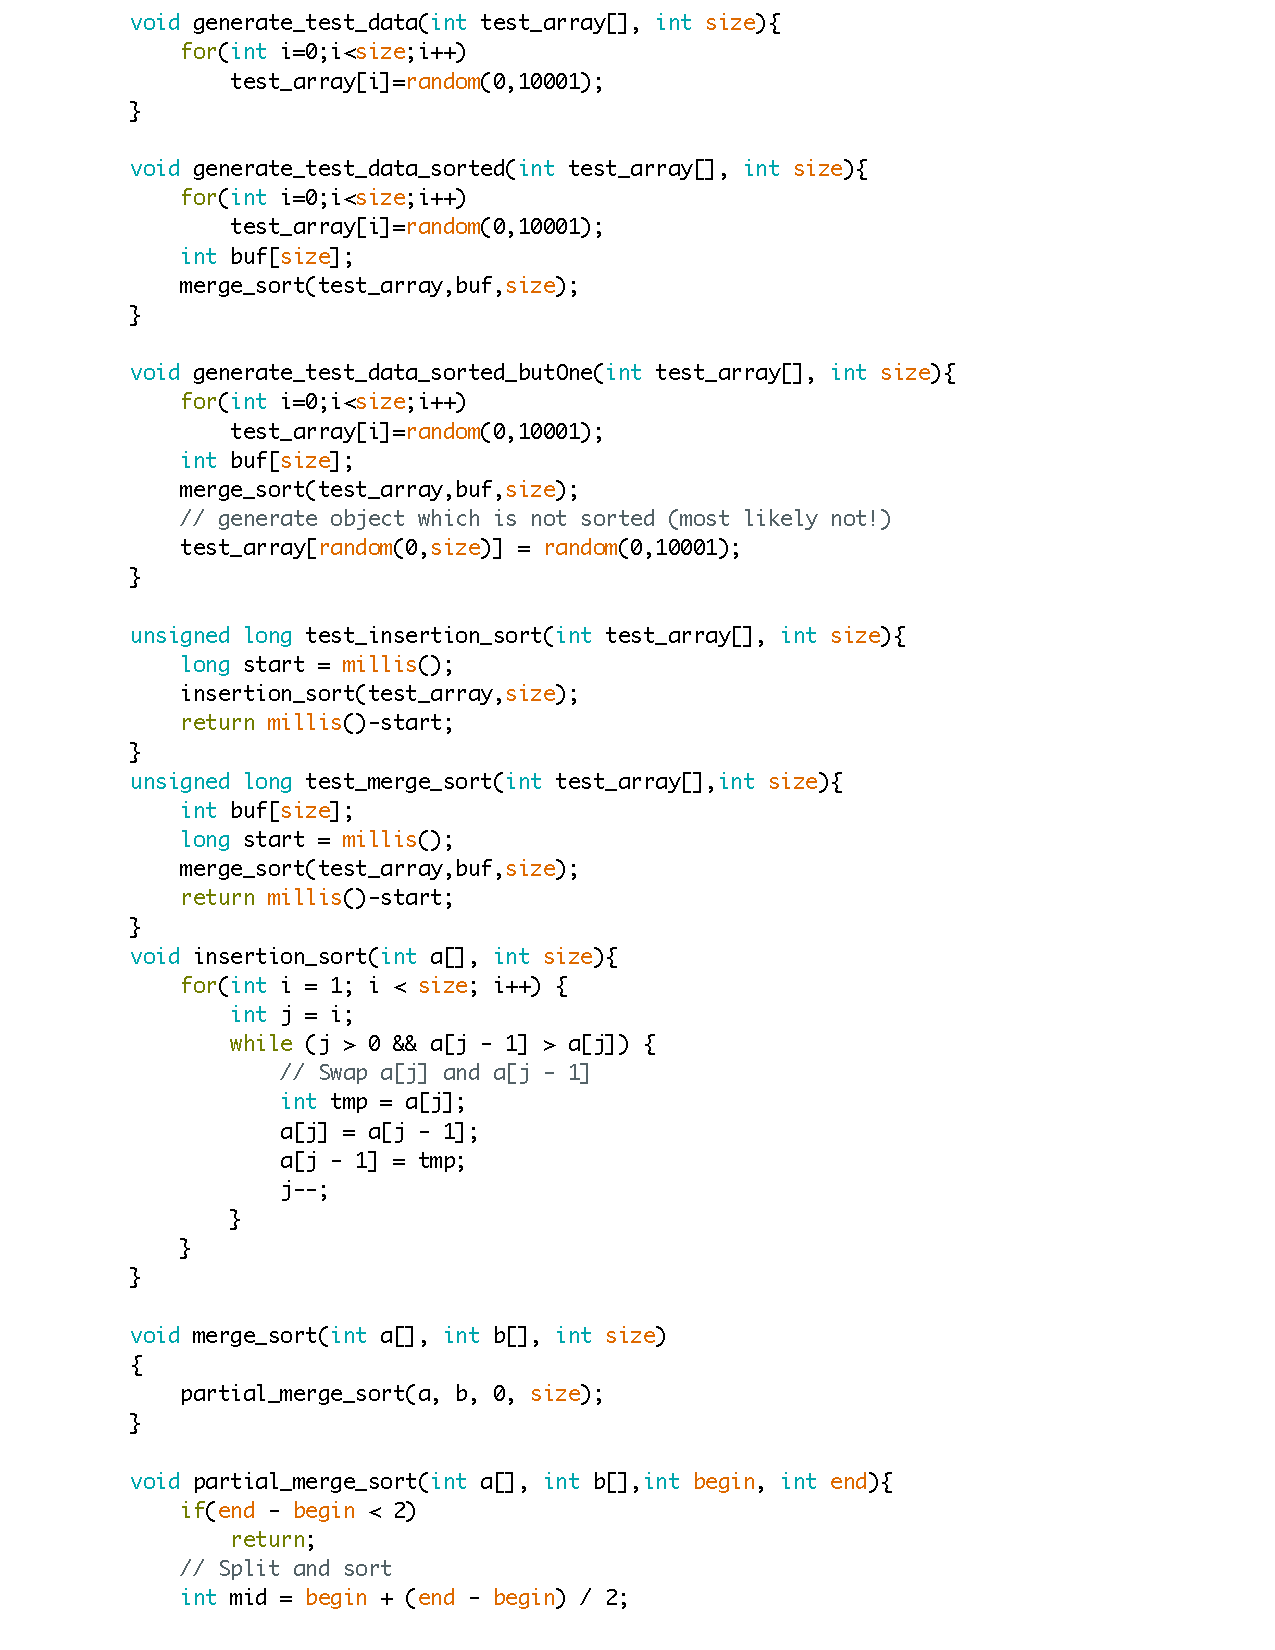
\includepdf[pages=-]{../Aufgabe2/Aufgabe2.pdf}



\end{document}
